% !TeX root = RJwrapper.tex
\title{Automating Reproducible, Collaborative Clinical Trial Document
Generation with the \pkg{listdown} Package}
\author{by Michael Kane, Xun Jiang, and Simon Urbanek}

\maketitle

\abstract{%
The conveyance of clinical trial explorations and analysis results from
a statistician to a clinical investigator is a critical component of the
drug development and clinical research cycle. Automating the process of
generating documents for data descriptions, summaries, exploration, and
analysis allows the statistician to provide a more comprehensive view of
the information captured by a clinical trial, and efficient generation
of these documents allows the statistican to focus more on the
conceptual development of a trial or trial analysis and less on the
implementation of the summaries and results on which decisions are made.
This paper explores the use of the \pkg{listdown} package for automating
reproducible documents in clinical trials that facilitate the
collaboration between statisticians and clinicians as well as defining
an analysis pipeline for document generation.
}

\hypertarget{background-and-introduction}{%
\section{Background and
Introduction}\label{background-and-introduction}}

The conveyance of clinical trial explorations and analysis results from
a statistician to a clinical investigator is an often overlooked but
critical component to the drug development and clinical research cycle.
Graphs, tables, and other analysis artifacts are at the nexus of these
collaborations. They facilitate identifying problems and bugs in the
data preparation and processing stage, they help to build an intuitive
understanding of mechanisms of disease and their treatment, they
elucidate prognostic and predictive relationships, they provide insight
that results in new hypotheses, and they convince researchers of
analyses testing hypotheses.

Despite their importance, the process of generating these artifacts is
usually done in an ad-hoc manner. This is partially because of the
nuance and diversity of the hypotheses and scientific questions being
interrogated and, to a lesser degree, the variation in clinical data
formatting. The usual process usually has a statistician providing a
standard set of artifacts, receiving feedback, and providing updates
based on feedback. Work performed for one trial is rarely leveraged on
others, and as a result, a large amount of work needs to be reproduced
for each trial.

There are two glaring problems with this approach. First, each analysis
of a trial requires a substantial amount of error-prone work. While the
variation between trials means some work needs to be done for
preparation, exploration, and analysis, many aspects of these trials
could be better automated resulting in greater efficiency and accuracy.
Second, because this work is challenging, it often occupies the majority
of the statisticians' effort. Less time is spent on trial design and
analysis, and then this portion is taken up by a clinician who often has
less expertise with the statistical aspects of the trial. As a result,
the extra effort spent on processing data undermines statisticians' role
as a collaborator and relegates them to service provider. Need tools
leveraging existing work to more efficiently provide holistic views on
trials will result in less effort and more accurate and comprehensive
trial design and analysis.

The richness of the \citet{R} package ecosystem, particularly with its
emphasis on analysis, visualization, reproducibility, and dissemination
makes the goal of creating these tools for clinical trials feasible.
Generation of tables is supported by packages including \pkg{tableone}
\citep{tableone}, \pkg{gt} \citep{gt}, \pkg{gtsummary}
\citep{gtsummary}. Visualization is achieved using package including
\pkg{ggplot2} \citep{ggplot2} and \pkg{survminer} \citep{survminer}. We
can even provide interactive presentations of data with \pkg{DT}
\citep{DT}, \pkg{plotly} \citep{plotly}, and \pkg{trelliscopejs}
\citep{trelliscopejs}.

It should also be realized that work building on these tools for
clinical trial data is already in process. The \pkg{greport}
\citep{greport} package provides graphical summaries for clinical trials
and has been used in conjunction with \pkg{rmarkdown} \citep{rmarkdown}
to produce specific trial report types with a specified format.

\hypertarget{using-for-programmatic-collaborative-clinical-trial-document-generation}{%
\section{\texorpdfstring{Using \pkg{listdown} for programmatic,
collaborative clinical trial document
generation}{Using  for programmatic, collaborative clinical trial document generation}}\label{using-for-programmatic-collaborative-clinical-trial-document-generation}}

The \pkg{listdown} package \citep{listdown} was recently released to
automate the process of generating reproducible (RMarkdown) documents.
Objects derived from a summary, exploration, or analysis are stored
hierarchically in an R \texttt{list}, which defines the structure of the
document. These objects are referred to as \emph{computational
components} since they are derived from computation, as opposed to
prose, which makes up the \emph{narrative components} of a document.

The computational components capture and structure the objects to be
presented. Describing how the objects will be presented and how the
document will be rendered is handled through the creation of a
\texttt{listdown} object. The separation between how computational
components are created and how they are shown to a user provides two
advantages. First, it decouples the data processing and analysis from
its exploration and visualization. For compute-intensive analyses, this
separation is critical for avoiding redundant computations for small
changes in the presentation. It also discourages putting
compute-intensive code into RMarkdown documents. Second, it provides the
flexibility to quickly change how a computational component is
visualized or summarized or even how a document is rendered. This makes
transitioning from an interactive .html document to a static .pdf
document significantly easier than substituting functions and parameters
in an R Markdown document.

The package has been found to be particularly useful in the reporting
and research of clinical trial data. In particular, the package has been
used for server collaborations focusing on either the analysis of past
trial data to formulate a new trial or in trial monitoring where trial
telemetry (enrollment, responses, etc.) is reported, and initial
analyses are conveyed to a clinician. The associated presentations
require very little context since clinicians often have as good an
understanding of the data collected as that of the statistician's
meaning narrative components are not needed. At the same time, a large
number of hierarchical, heterogeneous artifacts (tables and multiple
types of plots) can be automated where manual creation of RMarkdown
documents would be inconvenient and inefficient.

The rest of this document describes concepts implemented in the
\pkg{listdown} package for automated, reproducible document generation
and shows its use with a simplified, synthetic clinical trial data set
whose variables are typical of a non-small cell lung cancer trial. The
data set comes from the \pkg{forceps} \citep{forceps} package. As of the
time this document was written, the package is under development and is
not available on CRAN. However, it can be installed as follows.

\begin{Schunk}
\begin{Sinput}
devtools::install_github("kaneplusplus/forceps")
\end{Sinput}
\end{Schunk}

\noindent The following section uses the trial data to construct a
pipeline for document generation. We note that both the data and the
pipeline are simple when compared to most analyses of this type.
However, it is sufficient to illustrate accompanying concepts, and both
the analyses and concepts translate readily to real-world applications.
A final section discusses the use of the package and its current
direction.

\hypertarget{constructing-a-pipeline-for-document-generation}{%
\section{Constructing a pipeline for document
generation}\label{constructing-a-pipeline-for-document-generation}}

The process of analyzing data can be described using the classic
waterfall model of \citet{benington1983} where the output (the analysis
presentation or service) is dependent on a sequence of tasks that come
before it. This dependency structure means that if a problem is detected
in a given stage of the production of the analysis, all downstream parts
must be rerun to reflect the change. A graphical depiction of the
waterfall model, specific to data analyses (clinical or otherwise) is
shown in Figure \ref{fig:waterfall}. Note that data exploration and
visualization are an integral part of all stages of the production and
are often the means for identifying issues and refining analyses.

\begin{Schunk}
\begin{figure}[htbp]

{\centering 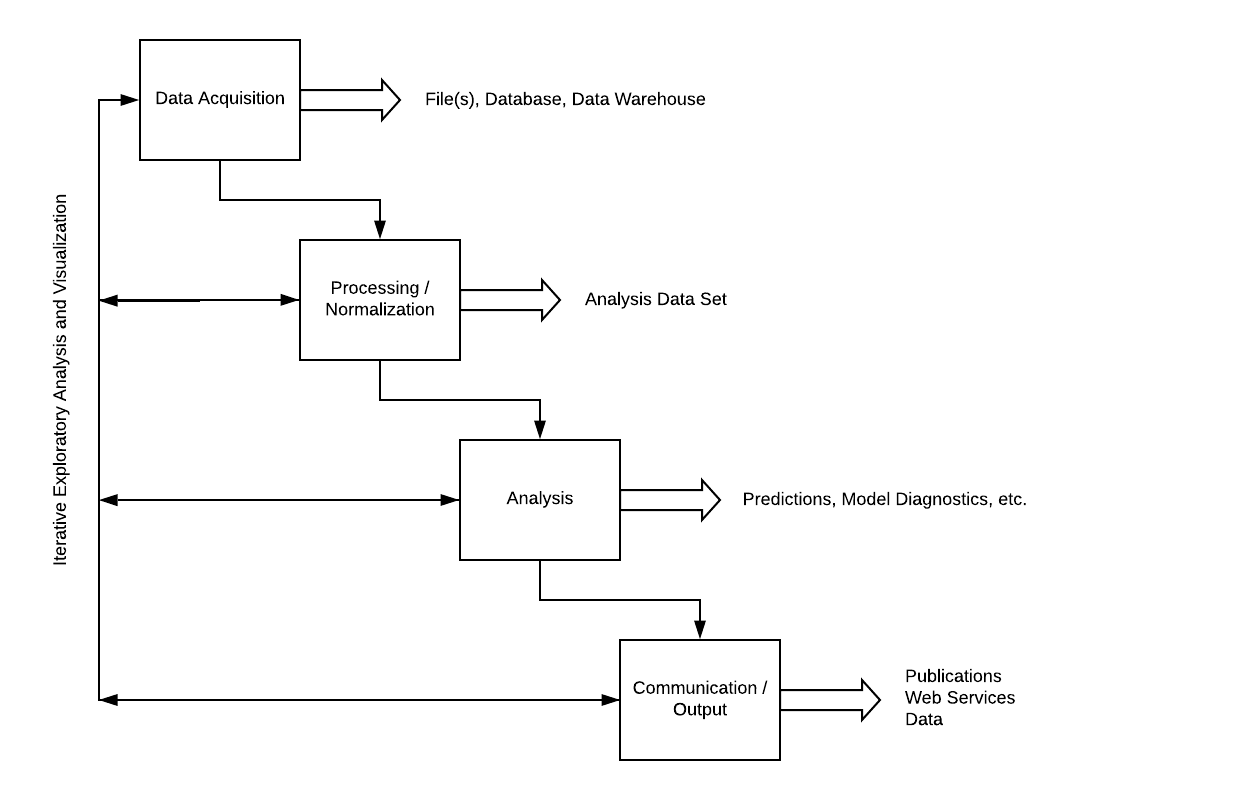
\includegraphics[width=5in]{waterfall} 

}

\caption[The data analysis waterfall]{The data analysis waterfall.}\label{fig:waterfall}
\end{figure}
\end{Schunk}

As explained in the previous section, we are going to implement a simple
analysis pipeline. The data acquisition and preprocessing steps are
handled by importing data sets from the \pkg{forceps} package and using
some of the functions implemented in the package to create a single
trial data set, thereby de-emphasizing these components in the pipeline.
While these steps are critical, the emphasis of this paper is the
incorporation of the \pkg{listdown} package into the later stages.

\hypertarget{data-acquisision-and-preprocessing}{%
\subsection{Data acquisision and
preprocessing}\label{data-acquisision-and-preprocessing}}

Data acquisition refers to the portion of the analysis pipeline where
the data is retrieved from some managed data store for integration into
the pipeline. These data sets may be retrieved as tables from a
database, case reports, Analysis Data Model (ADaM) data formatted
according to the Clinical Data Interchange Standards Consortium (CDISC)
\citep{CDISC}, Electronic Health Records, or other clinical Real World
Data (RWD) formats. These data are then transformed to a format
appropriate for analysis.

In our simple example, this is accomplished by loading data
corresponding to trial outcomes, patient adverse events, patient
biomarkers, and patient demography and transforming them into a single
data set with one row per patient and one variable per column using the
\pkg{forceps} and \pkg{dplyr} \citep{dplyr} packages. The data also
includes longitudinal adverse event information, which will is stored as
a nested data frame in the \texttt{ae\_long} column of the resulting
data set.

\begin{Schunk}
\begin{Sinput}
library(forceps)
library(dplyr)

data(lc_adsl, lc_adverse_events, lc_biomarkers, lc_demography)

lc_trial <- consolidate(
  list(adsl = lc_adsl,
       adverse_events = lc_adverse_events %>% 
         cohort(on = "usubjid", name = "ae_long"),
       biomarkers = lc_biomarkers,
       demography = lc_demography %>% 
         select(-chemo_stop)
  ),
  on = "usubjid")

lc_trial
\end{Sinput}
\begin{Soutput}
#> # A tibble: 558 x 18
#>    usubjid best_response   pfs_d~1 pfs_c~2 os_days os_ce~3 chemo~4 arm   ae_co~5
#>      <dbl> <chr>             <dbl>   <dbl>   <dbl>   <dbl> <chr>   <chr>   <int>
#>  1    1003 Stable Disease      101       1     233       1 advers~ stan~      15
#>  2    1005 Complete Respo~      78       0     184       1 advers~ stan~      19
#>  3    1006 Progressive Di~     253       1     333       1 treatm~ stan~      11
#>  4    1009 Partial Respon~     130       0     643       0 <NA>    trea~      12
#>  5    1014 Complete Respo~      41       1     116       1 advers~ trea~       5
#>  6    1018 Partial Respon~     194       1     423       1 treatm~ stan~      10
#>  7    1023 Stable Disease       49       1     337       1 advers~ stan~       1
#>  8    1025 Stable Disease       95       1     589       1 advers~ stan~      13
#>  9    1030 Complete Respo~     351       1     688       1 advers~ stan~      25
#> 10    1033 Complete Respo~      33       1     125       1 treatm~ stan~       6
#> # ... with 548 more rows, 9 more variables: ae_long <list>,
#> #   egfr_mutation <chr>, smoking <chr>, ecog <chr>, prior_resp <chr>,
#> #   site_id <int>, sex <chr>, refractory <lgl>, age <dbl>, and abbreviated
#> #   variable names 1: pfs_days, 2: pfs_censor, 3: os_censor, 4: chemo_stop,
#> #   5: ae_count
#> # i Use `print(n = ...)` to see more rows, and `colnames()` to see all variable names
\end{Soutput}
\end{Schunk}

\hypertarget{analysis-defining-and-structuring-the-computational-components}{%
\subsection{Analysis defining and structuring the computational
components}\label{analysis-defining-and-structuring-the-computational-components}}

The next step is to define the computational components as a
hierarchical, named list of objects that will be presented. These
objects are generally derived from the exploratory, descriptive, and
analysis stages and are presented as visualizations and tables. This
example will focus on the exploratory and descriptive portions. We will
start by defining a new function \texttt{class\_and\_tag()}, which takes
an object and prepends a class designation to the objects along with
optionally associating the object with a set of attributes. This extra
information will be used later in order to dispatch to the proper
functions responsible for presenting the objects in a resulting R
Markdown document. If no such information is given, then the object will
be presented as it usually would in the document. It should also be
noted that \texttt{class\_and\_tag()} is provided for convenience here
and will be available in subsequent package versions.

The next step is to define the computational components that will be
presented. Our simple example will contain three sections: Outcome
Information, Adverse Events, Biomarkers. The Adverse Events and
Biomarkers sections will each show summary tables of one of the
variables from those data. The Outcome Information section will be
composed of two subsections, with the first (Best Response) providing a
summary of the best response by the arm and the second (Overall
Survival) showing a survival plot by arm of the overall survival. The
call to \texttt{ld\_cc\_dendro()} at the end of the example provides of
dendrogram of the hierarchical structure.

\begin{Schunk}
\begin{Sinput}
library(listdown)

trial_summary <- list(
  `Outcome Information` = list(
    `Best Response` = lc_trial %>% 
      select(best_response, arm) %>% 
      class_and_tag("summary_table", by = "arm"),
    `Overall Survival` = lc_trial %>% 
      select(os_days, os_censor, arm) %>% 
      class_and_tag("survival_plot", 
                    time = "os_days", 
                    censor = "os_censor", 
                    x = "arm")),
  `Adverse Events` = lc_trial %>%
    select(best_response) %>%
    class_and_tag("summary_table"),
  `Biomarkers` = list(
    `EGFR` = lc_trial %>%
      select(egfr_mutation) %>%
      class_and_tag("summary_table")
  )
)

ld_cc_dendro(trial_summary)
\end{Sinput}
\begin{Soutput}
#> 
#> trial_summary
#>   |-- Outcome Information
#>    |-- Best Response
#>    |  o-- object of type(s):summary_table tbl_df tbl data.frame
#>    o-- Overall Survival
#>       o-- object of type(s):survival_plot tbl_df tbl data.frame
#>   |-- Adverse Events
#>   |  o-- object of type(s):summary_table tbl_df tbl data.frame
#>   o-- Biomarkers
#>    o-- EGFR
#>       o-- object of type(s):summary_table tbl_df tbl data.frame
\end{Soutput}
\end{Schunk}

\hypertarget{communicating-results}{%
\subsection{Communicating results}\label{communicating-results}}

The objects have been constructed and they have been structured. The
next step is to define how they will be presented. This is done by
creating two functions \texttt{make\_summary} and
\texttt{make\_survival\_plot}. The former takes a \texttt{data.frame}
and uses the \pkg{gtsummary} package to summarize the results. If the
\texttt{data.frame} includes an attribute named \texttt{by} and denoting
a valid variable in the data set, then the summary is created
conditionally on that variable. The latter function also takes a
\texttt{data.frame} and uses attributes to denote variables on which a
Kaplan-Meier plot can be constructed using the \pkg{survival}
\citep{survival} and \pkg{survminer} packages. The functions are written
to a file called \texttt{decorators.r} and will be used by the R
Markdown document to render the final document.

\begin{Schunk}
\begin{Sinput}
library(gtsummary)
library(survival)
library(survminer)
library(dplyr)

make_summary <- function(x) {
  by <- attributes(x)$by
  tbl_summary(x, by = by)
}

make_survival_plot <- function(.x) {
  att <- attributes(.x)
  x <- ifelse(is.null(att$x), "1", att$x)
  form <- sprintf("Surv(%s, %s) ~ %s", att$time, att$censor, x) %>%
    as.formula()
  fit <- surv_fit(form, data = as.data.frame(.x))
  ggsurvplot(fit, data = as.data.frame(.x))
}
\end{Sinput}
\end{Schunk}

The next step is to connect the computational components to the
functions that will present them using the \texttt{listdown()} function.
First, the computational components are stored in the
\texttt{trial\_summary} object are written to the disk. The resulting R
Markdown document will read it in based on the \texttt{load\_cc\_expr}
argument. Along with reading in the data, initialization in the R
Markdown document will include sourcing the \texttt{decorators.r} file
previously written to disk. This is handled with the \texttt{init\_expr}
argument. The \texttt{decorators} argument takes a list where the name
specifies the class and the list element corresponds to a function that
will present objects of the specified class. For example,
\texttt{summary\_table} objects are sent to the \texttt{make\_summary()}
function for presentation. This allows us to connect objects to their
appropriate function to process and present them. Finally, \texttt{echo}
and \texttt{message} chunk options are set to \texttt{FALSE} so that the
code and associated messages will not appear in the final rendered
document. The last line of code below displays the first 12 lines of R
Markdown code chunks as they will appear in the corresponding document.

\begin{Schunk}
\begin{Sinput}
saveRDS(trial_summary, "cc.rds")

ld <- listdown(load_cc_expr = readRDS("cc.rds"),
               init_expr = source("decorators.r"),
               decorator = list(summary_table = make_summary,
                                survival_plot = make_survival_plot),
               echo = FALSE,
               message = FALSE)

ld_make_chunks(ld)[1:12]
\end{Sinput}
\begin{Soutput}
#>  [1] ""                                    
#>  [2] "```{r echo = FALSE, message = FALSE}"
#>  [3] "source(\"decorators.r\")"            
#>  [4] ""                                    
#>  [5] "cc_list <- readRDS(\"cc.rds\")"      
#>  [6] "```"                                 
#>  [7] ""                                    
#>  [8] "# Outcome Information"               
#>  [9] ""                                    
#> [10] "## Best Response"                    
#> [11] ""                                    
#> [12] "```{r echo = FALSE, message = FALSE}"
\end{Soutput}
\end{Schunk}

The last step creates the R Markdown header, writes it along with the R
code chunks to a file named \texttt{"simple-data-trial-summary.rmd"} and
knits the file with the \pkg{knitr} package \citep{knitr} to a pdf
document, per the \texttt{output} argument of the
\texttt{ld\_rmarkdown\_header()} function. \texttt{md\_header} is a
\texttt{yml} object making it easy to control how the document is
rendered. The code to generate the document along with the resulting R
Markdown and output file constitute a reproducible workflow that can be
quickly iterated upon and adapted for different types of explorations,
summaries, and analyses.

\begin{Schunk}
\begin{Sinput}
library(knitr)

md_header <- ld_rmarkdown_header("Fake Data Trial Summary",
                                 output = "pdf_document")

ld_write_file(
  rmd_header = as.character(md_header),
  ld = ld_make_chunks(ld),
  file_name = "simple-data-trial-summary.rmd")

knit("simple-data-trial-summary.rmd")
\end{Sinput}
\end{Schunk}

\hypertarget{direction}{%
\section{Direction}\label{direction}}

The \pkg{listdown} package has been successfully used for collaborations
on several clinical trial analyses. The package works particularly well
when creating large, navigable sets of summaries and visualizations.
Current work focuses on two areas. First is the construction of standard
decorators. By packaging decorators and associated functionality,
presentations can be made rich as they are developed over time. This
standardization also makes it easier to leverage work in configuring
chunks so that they can be made more aesthetic by default. In addition,
we have been working on abstract and formalize the notion of document
composition. In the example presented, the aggregation of the header and
R code chunks into a file was sufficient for generating a document.
However, the composition of other outputs is also supported. For
example, the top-level names of the trial summary could just as easily
designate tabs on a web page or other target. The notion of a composer
would allow a user to target a greater variety of output types, better
suiting the application under consideration and the target audience for
the presentation.

\bibliography{listdown.bib}

\address{%
Michael Kane\\
Yale University\\%
60 College Street\\ New Haven, CT 06510, USA\\
%
%
%
\href{mailto:michael.kane@yale.edu}{\nolinkurl{michael.kane@yale.edu}}%
}

\address{%
Xun Jiang\\
Amgen Inc.\\%
One Amgen Center Drive\\ Thousand Oaks, CA 91320-1799, USA\\
%
%
%
\href{mailto:xunj@amgen.com}{\nolinkurl{xunj@amgen.com}}%
}

\address{%
Simon Urbanek\\
The University of Aukland\\%
38 Princes Street\\ Auckland Central, Aukland 1010, NZ\\
%
%
%
\href{mailto:s.urbanek@auckland.ac.nz}{\nolinkurl{s.urbanek@auckland.ac.nz}}%
}
